
\chapter[Tán sắc ánh sáng]{Tán sắc ánh sáng}
\section{Lý thuyết}

\subsection{Nhắc lại lăng kính}
\subsubsection{Đường truyền của tia sáng qua lăng kính}
Khi tia sáng được chiếu đến lăng kính, tia sáng sẽ bị khúc xạ ở các mặt bên như hình vẽ. 
\begin{center}
	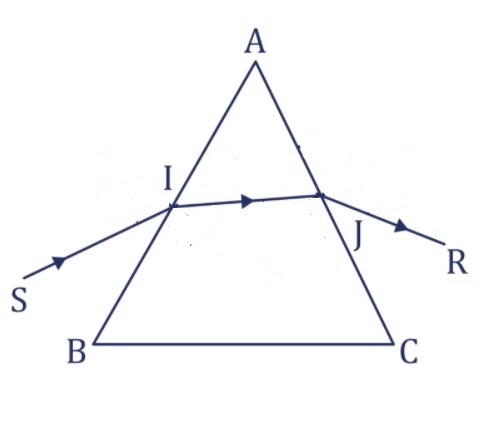
\includegraphics[scale=0.4]{../figs/VN12-PH-32-L-019-1-1.jpg}
\end{center}

Góc tạo bởi tia ló và tia tới gọi là \textit{góc lệch $D$} của ánh sáng khi truyền qua lăng kính.
\manatip{Khi không xảy ra phản xạ toàn phần, tia ló bao giờ cũng lệch về phía đáy lăng kính.}	
\subsubsection{Công thức của lăng kính}
\begin{center}
	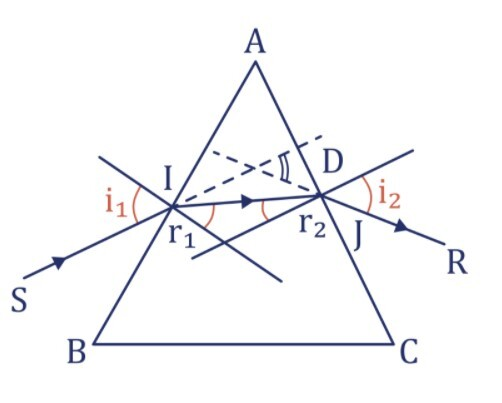
\includegraphics[scale=0.45]{../figs/VN12-PH-32-L-019-1-2.jpg}
\end{center}
\begin{itemize}
	\item Tại I: $\sin i_1=n\sin r_1$.
	\item Tại J: $\sin i_2=n\sin r_2$.
	\item Góc chiết quang: $A=r_1+r_2$.
	\item Góc lệch của tia sáng qua lăng kính: $D=i_1+i_2-A$.
\end{itemize}

\luuy{
	Nếu các góc nhỏ hơn $10^\circ$ thì công thức gần đúng của lăng kính là:
	\begin{itemize}
		\item $i_1=nr_1$,
		\item $i_2=nr_2$,
		\item $A=r_1=r_2$,
		\item $D=(n-1)A$.
	\end{itemize}
}

\subsection{Sự tán sắc ánh sáng}
\begin{center}
	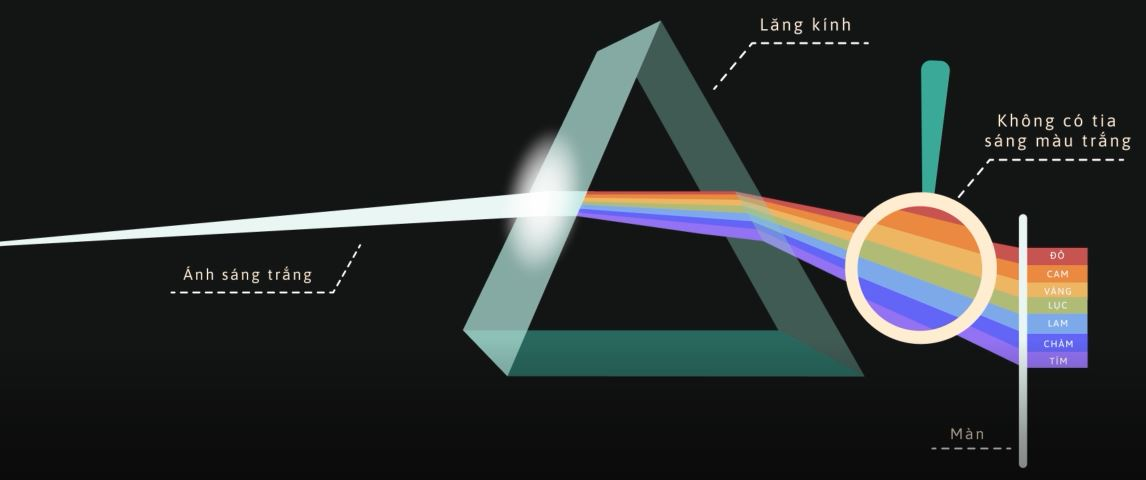
\includegraphics[width=\linewidth]{../figs/VN12-PH-32-L-019-1-3.jpg}
\end{center}

\begin{description}
	
	\item[Sự tán sắc ánh sáng] là sự phân tách một chùm sáng phức tạp thành các chùm sáng đơn sắc.
	\item[Ánh sáng đơn sắc] là ánh sáng có một màu nhất định và không bị tán sắc khi qua lăng kính.
	\item[Ánh sáng trắng] là hỗn hợp của nhiều ánh sáng đơn sắc có màu biến thiên liên tục từ màu đỏ đến màu tím. 
	\item[Chiết suất của thủy tinh] đối với các ánh sáng đơn sắc khác nhau thì khác nhau. Chiết suất có giá trị nhỏ nhất đối với ánh sáng đỏ và tăng dần khi chuyển sang màu da cam, màu vàng, ... và có giá trị lớn nhất đối với ánh sáng tím. Đặc điểm này là chung cho mọi chất trong suốt ($n_{\text{đ}}\leq n \leq  n_{\text{t}} $).
\end{description}

%		\luuy{ Mỗi ánh sáng đơn sắc có một tần số xác định}

\section{Bài tập tự luyện}
\begin{enumerate}[label=\bfseries Câu \arabic*:]
	
	%========================================
	\item \mkstar{1} [2]
	\cauhoi
	{Trong chân không, một ánh sáng đơn sắc có tần số $4\cdot 10^{14}\ \text {Hz}$. Biết chiết suất của ánh sáng này trong nước là $4/3$. Tần số của ánh sáng này trong nước là
		\begin{mcq}(4)
			\item $\text{5,3}\cdot 10^{14}\ \text{Hz}$. 
			\item $\text{3,0} \cdot10^{14}\ \text{Hz}$. 
			\item $\text{4,0} \cdot10^{14}\ \text{Hz}$. 
			\item $\text{3,4}\cdot10^{14}\ \text{Hz}$. 
		\end{mcq}
	}
	
	\loigiai
	{		\textbf{Đáp án: C.}
		
		Khi truyền từ môi trường này sang môi trường khác, tần số ánh sáng là không đổi.		
		
	}
	
	%========================================

	

	
	%========================================
	\item \mkstar{1} [7]
	\cauhoi
	{Hiện tượng tán sắc ánh sáng thực chất là hiện tượng
		\begin{mcq}(1)
			\item tạo thành chùm ánh sáng trắng từ sự hoà trộn của các chùm ánh sáng đơn sắc.
			\item tạo thành chùm ánh sáng đơn sắc từ sự phân tích chùm ánh sáng trắng.
			\item đổi màu của các tia sáng.
			\item chùm sáng trắng bị mất đi một số màu.
		\end{mcq}
	}
	
	\loigiai
	{		\textbf{Đáp án: B.}
		
		Hiện tượng tán sắc ánh sáng thực chất là hiện tượng tạo thành chùm ánh sáng đơn sắc từ sự phân tích chùm ánh sáng trắng.
		
	}
	
	%========================================
	\item \mkstar{1} [7]
	\cauhoi
	{Cầu vồng là kết quả của hiện tượng
		\begin{mcq}(2)
			\item tán sắc ánh sáng. 
			\item nhiễu xạ ánh sáng. 
			\item khúc xạ ánh sáng. 
			\item giao thoa ánh sáng. 
		\end{mcq}
	}
	
	\loigiai
	{		\textbf{Đáp án: A.}
		
		Cầu vồng là kết quả của hiện tượng tán sắc ánh sáng.
		
	}
	
	%========================================
	\item \mkstar{1} [10]
	\cauhoi
	{Khi một chùm ánh sáng song song, hẹp truyền qua một lăng kính thì bị phân tách thành các chùm sáng đơn sắc khác nhau. Đây là hiện tượng
		\begin{mcq}(2)
			\item giao thoa ánh sáng. 
			\item tán sắc ánh sáng. 
			\item nhiễu xạ ánh sáng. 
			\item phản xạ ánh sáng. 
		\end{mcq}
	}
	
	\loigiai
	{		\textbf{Đáp án: B.}
		
		Khi một chùm ánh sáng song song, hẹp truyền qua một lăng kính thì bị phân tách thành các chùm sáng đơn sắc khác nhau. Đây là hiện tượng tán sắc ánh sáng.
		
	}
	
	%=======================	
	\item \mkstar{1} [1]
	\cauhoi
	{Chiết suất của một môi trường trong suốt đối với các ánh sáng đơn sắc đỏ, lục, tím lần lượt là $n_{d}, n_{l}, n_{t}$. Quan hệ nào sau đây là \textbf{đúng}?
		\begin{mcq}(2)
			\item $n_{l} > n_{d} > n_{t}$. 
			\item $n_{d} < n_{l} < n_{t}$. 
			\item $n_{d} > n_{l} > n_{t}$. 
			\item $n_{l} < n_{d} < n_{t}$. 
		\end{mcq}
	}
	
	\loigiai
	{		\textbf{Đáp án: B.}
		
		Ánh sáng màu tím có chiết suất lớn nhất, màu đỏ nhỏ nhất. Nên mối quan hệ đúng là
		$$
		n_{d} < n_{l} < n_{t}.
		$$
		
	}
	
	%========================================

	
	%========================================
	\item \mkstar{1} [4]
	\cauhoi
	{Gọi $n_{d}, n_{t}$ và $n_{v}$ lần lượt là chiết suất của một môi trường trong suốt đối với các ánh sáng đơn sắc đỏ, tím và vàng. Sắp xếp nào sau đây là đúng?
		\begin{mcq}(2)
			\item $n_{d} < n_{v} < n_{t}$. 
			\item $n_{v} > n_{d} > n_{t}$. 
			\item $n_{d} > n_{t} > n_{v}$. 
			\item $n_{t} > n_{d} > n_{v}$. 
		\end{mcq}
	}
	
	\loigiai
	{		\textbf{Đáp án: A.}
		
		Ánh sáng màu đỏ có chiết suất nhỏ nhất và ánh sáng màu tìm có chiết suất lớn nhất nên sắp xếp đúng là
		$$
		n_{d} < n_{v} < n_{t}.
		$$
		
	}
	
	%========================================

	
	%========================================
	\item \mkstar{2} [2]
	\cauhoi
	{Chiếu xiên góc lần lượt bốn ánh sáng đơn sắc màu cam, màu lam, màu vàng, màu chàm từ không khí vào nước với cùng một góc tới. So với phương của tia tới, tia khúc xạ bị lệch ít nhất là tia màu
		\begin{mcq}(4)
			\item chàm. 
			\item cam. 
			\item vàng. 
			\item lam. 
		\end{mcq}
	}
	
	\loigiai
	{		\textbf{Đáp án: B.}
		
		Tia bị lệch ít nhất là tia có chiết suất nhỏ nhất. Vậy nên tia màu cam bị lệch ít nhất.
		
	}
	
	%========================================
	\item \mkstar{2} [3]
	\cauhoi
	{Chiếu xiên một chùm sáng hẹp gồm bốn ánh sáng đơn sắc đỏ, vàng, lam, tím từ trong nước ra không khí. Khi tia màu lam nằm là là mặt phân cách giữa hai môi trường thì
		\begin{mcq}(1)
			\item hai ánh sáng đỏ và tím bị phản xạ toàn phần. 
			\item so với phương tia tới, tia khúc xạ đỏ bị lệch ít hơn tia khúc xạ vàng.
			\item tia khúc xạ chỉ là ánh sáng tím, còn tia sáng đỏ và vàng bị phản xạ toàn phần. 
			\item so với phương tia tới, tia khúc xạ vàng bị lệch ít hơn tia khúc xạ đỏ. 
		\end{mcq}
	}
	
	\loigiai
	{		\textbf{Đáp án: B.}
		
		Khi tia màu lam nằm là là mặt phân cách giữa hai môi trường thì tia màu đỏ và vàng bị khúc xạ, còn tia màu tím bị phản xạ toàn phần.\\
		Do chiết suất của ánh sáng màu đỏ nhỏ hơn chiết suất của ánh sáng màu vàng nên so với phương tia tới, tia khúc xạ đỏ bị lệch ít hơn tia khúc xạ vàng.
		
	}
	
	%========================================
	\item \mkstar{2} [7]
	\cauhoi
	{Gọi $n_{c}, n_{l}, n_{L}, n_{v}$ lần lượt là chiết suất của thủy tinh đối với các tia chàm, lam, lục và vàng. Sắp xếp theo thứ tự nào dưới đây là đúng
		\begin{mcq}(2)
			\item $n_{c} > n_{L} > n_{l} > n_{v}$. 
			\item $n_{c} < n_{L} < n_{l} < n_{v}$. 
			\item $n_{c} < n_{l} < n_{L} < n_{v}$. 
			\item $n_{c} > n_{l} > n_{L} > n_{v}$. 
		\end{mcq}
	}
	
	\loigiai
	{		\textbf{Đáp án: D.}
		
		Trong các màu theo sắp xếp đỏ, cam, vàng, lục, lam, chàm, tím thì màu tím có chiết suất lớn nhất và màu đỏ nhỏ nhất. Vậy nên sắp xếp đúng phải là
		$$
		n_{c} > n_{l} > n_{L} > n_{v}.
		$$
		
	}
		\item \mkstar{1} 
	\cauhoi
	{Một ánh sáng đơn sắc tần số $f$ truyền trong một môi trường với vận tốc $v$ thì nó có bước sóng bằng
		
		\begin{mcq}(4)
			\item $\lambda = v \cdot f.$
			\item $\lambda = \dfrac{v}{f}.$
			\item $\lambda = \dfrac{f}{v}.$
			\item $\lambda = 2vf.$
		\end{mcq}
	}
	
	\loigiai
	{		\textbf{Đáp án: B.}
		
	
		
	}
		\item \mkstar{1} 
	\cauhoi
	{
		Một ánh sáng đơn sắc truyền trong một môi trường với vận tốc $v$ thì chiết suất tuyệt đối của môi trường với ánh sáng đó là
		
		\begin{mcq}(4)
			\item $n = \dfrac{c}{v}.$
			\item $n = c \cdot v.$
			\item $n = \dfrac{v}{c}.$
			\item $n = \dfrac{2c}{v}.$
		\end{mcq}
	}
	
	\loigiai
	{		\textbf{Đáp án: A.}
		
		
		
	}
	\item \mkstar{1} 
	\cauhoi
	{
		Một ánh sáng đơn sắc truyền từ chân không có bước sóng $\lambda_0$ vào một môi trường có chiết suất tuyệt đối $n$ (đối với ánh sáng đó) thì bước sóng $\lambda$ của ánh sáng đơn sắc đó trong môi trường này là
		
		
		\begin{mcq}(4)
			\item $\lambda = c\lambda_0$.
			\item $\lambda = n\lambda_0$.
			\item $\lambda = \dfrac{\lambda_0}{n}.$
			\item $\lambda = \lambda_0$.
		\end{mcq}
	}
	
	\loigiai
	{		\textbf{Đáp án: C.}
		
		
		
	}
		\item \mkstar{1} 
	\cauhoi
	{Chiếu chùm sáng hẹp đơn sắc song song màu vàng theo phương vuông góc với mặt bên của một lăng kính thì tia ló đi là là trên mặt bên thứ hai của lăng kính. Nếu thay bàng chùm sáng gồm bốn ánh sáng đơn sắc: đỏ, cam, lục và tím thì các tia ló ra khỏi lăng kính ở mặt bèn thứ hai
		
		\begin{mcq}
			\item tia cam và tia đỏ.	
			\item tia cam và tím.
			\item tia tím, lục và cam.	
			\item tia lục và tím.
		\end{mcq}
	}
	
	\loigiai
	{		\textbf{Đáp án: A.}
		
		Tia vàng là là mặt bên thứ hai và $n_\text t > n_\text l > n_\text v>n_\text c>n_\text{đ}$ nên tia đỏ và cam có thể ló ra khỏi lăng kính ở mặt bên thứ hai.
		
	}
		\item \mkstar{1} 
	\cauhoi
	{
		Khi một chùm sáng đơn sắc truyền từ không khí vào thủy tinh thì
		
		\begin{mcq}
			\item màu sắc thay đổi, tần số không đổi, bước sóng giảm.
			\item màu sắc thay đổi, tần số không đổi, bước không đổi.
			\item màu sắc không đổi, tần số không đổi, bước sóng giảm.
			\item màu sắc không đổi, tần số không đổi, bước sóng tăng.
		\end{mcq}
	}
	
	\loigiai
	{		\textbf{Đáp án: C.}
		
		Khi ánh sáng đơn sắc truyền từ không khí vào thuỷ tinh thì màu sắc không đổi, tần số không đổi, bước sóng giảm. 
		
	}
		\item \mkstar{2} 
	\cauhoi
	{
		Ánh sáng lam có bước sóng trong chân không và trong nước lần lượt là $\SI{0,4861}{\mu m}$ và $\SI{0,3635}{\mu m}$. Chiết suất tuyệt đối của nước đối với ánh sáng lam là
		
		\begin{mcq}(4)
			\item 1,3335.
			\item 1,3725.
			\item 1,3301.
			\item 1,3373.
		\end{mcq}
	}
	
	\loigiai
	{		\textbf{Đáp án: D.}
		
		Chiết suất tuyệt đối của nước đối với ánh sáng lam
		
		$$\lambda = \dfrac{v}{f} = \dfrac{c}{nf} \Rightarrow \dfrac{n_\text{nước}}{n_\text{ck}}= \dfrac{\lambda_\text{ck}}{\lambda_\text{nước}} = \text{1,3373} \Rightarrow n_\text{nước} = \text{1,3373}.$$
		
	}
		\item \mkstar{2} 
	\cauhoi
	{Ánh sáng đơn sắc $\lambda = \SI{0,6}{\mu m}$ trong chân không. Tốc độ và bước sóng khi ánh sáng truyền trong thủy tinh có chiết suất $n =$ 1,5 lần lượt bằng
		
		
		\begin{mcq}(2)
			\item $2\cdot 10^8\ \text{m/s}; \SI{0,4}{\mu m}.$
			\item $10^8\ \text{m/s}; \SI{0,67}{\mu m}.$
			\item $\text{1,5}\cdot 10^8\ \text{m/s}; \SI{0,56}{\mu m}.$
			\item $\text{2,3}\cdot 10^8\ \text{m/s}; \SI{0,38}{\mu m}.$
		\end{mcq}
	}
	
	\loigiai
	{		\textbf{Đáp án: A.}
		
		Ta có:
		
		$$ n =\dfrac{c}{v}  \Rightarrow v = \dfrac{c}{n} = 2\cdot 10^8\ \text{m/s}.$$
		
		Khi truyền từ môi trường này sang môi trường khác thì tần số của ánh sáng là không đổi. Bước sóng của ánh sáng khi truyền trong chân không:
		
		$$\lambda_0 = \dfrac{c}{f}.$$
		
		Bước sóng của ánh sáng khi truyền trong môi trường có chiết suất $n$:
		
		$$\lambda = \dfrac{v}{f} = \dfrac{\lambda_0}{n} \Rightarrow \lambda = \SI{0,4}{\mu m}.$$
		
		
	}
	
\end{enumerate}











